% This is samplepaper.tex, a sample chapter demonstrating the
% LLNCS macro package for Springer Computer Science proceedings;
% Version 2.20 of 2017/10/04
%
\documentclass[runningheads]{llncs}
%
\usepackage{graphicx}
\usepackage{amsmath}
\usepackage{amsfonts}
\usepackage{float}
% Used for displaying a sample figure. If possible, figure files should
% be included in EPS format.
%
% If you use the hyperref package, please uncomment the following line
% to display URLs in blue roman font according to Springer's eBook style:
% \renewcommand\UrlFont{\color{blue}\rmfamily}

\begin{document}
%
\title{Dual watermarking scheme for handwritten document image integrity, tamper detection and copyright protection}
%
%\titlerunning{Abbreviated paper title}
% If the paper title is too long for the running head, you can set
% an abbreviated paper title here
%
\author{Ernesto Avila-Domenech\inst{1}\orcidID{0000-0002-4797-289X} \and
Alberto Taboada-Crispi\inst{2}\orcidID{0000-0002-7797-1441} \and
Anier Soria-Lorente\inst{1}\orcidID{0000-0003-3488-3094}}
%
\authorrunning{E. Avila-Domenech et al.}
% First names are abbreviated in the running head.
% If there are more than two authors, 'et al.' is used.
%
\institute{Universidad de Granma, Carretera Central v{\'i}a Holgu{\'i}n Km $\frac{1}{2}$, Granma, Cuba \email{\{eadomenech, asorial1983\}@gmail.com}\\ \and
Universidad Central de Las Villas, Villa Clara, Cuba\\
\email{\{abc,lncs\}@uni-heidelberg.de}}
%
\maketitle              % typeset the header of the contribution
%
\begin{abstract}
In this paper, by using SHA-256 hash function, a fragile watermarking for handwritten document image integrity and tamper detection method is proposed. In this paper, we propose a watermarking scheme called “dual watermarking”. Dual watermark is a combination of a visible watermark and an invisible watermark.

\keywords{First keyword  \and Second keyword \and Another keyword.}
\end{abstract}
%
%
%
\section{Introduction}
The explosive growth of digital multimedia techniques, together with the rapid development of digital network communication has created a pressing demand for techniques that can be used for copy protection, copyright protection and content authentication. Owing to the need of copyright protection and authentication validation, Digital Rights Management (DRM) is gaining importance. DRM refers to a range of access control technologies used to limit or restrict usage of digital content. Digital watermarking is useful in DRM systems as it can hide information within the digital content like images, audio and video.

In \cite{mohanty1999dual} is presented a dual watermarking technique which attempts to establish the owner’s right to the image and detect the intentional and unintentional tampering of the image. However, this early research is simply a combination of visible and invisible watermarking algorithms.

Many types of watermarking techniques have been developed for a variety of applications.

To solve this problem, methods are developed that can be classified into digital signature-based methods and watermarking-based methods.

A digital signature is a set of features extracted from an image and these are stored in a separate file. Digital watermarking consists of inserting imperceptible information called watermark in a multimedia document to protect the copyright of the document while ensuring its effective transmission \cite{el2014image}.

Watermarks may be visible or invisible, where a visible mark is easily detected by observation while an invisible mark is designed to be transparent to the observer and detected using signal processing techniques.

A robust mark is designed to resist attacks that attempt to remove or destroy the mark. Such attacks include lossy compression, filtering, and geometric scaling. A fragile mark is designed to detect slight changes to the watermarked image with high probability.

The main application of fragile watermarks is in content authentication.

Different with the robust image watermarking that is robust to a variety of attacks for ownership and copyright protection, fragile image watermarking is utilized for the integrity authentication, which is fragile to the illegal tampering.

The main application of fragile watermarks is in content authentication. That is, it may be of interest for parties to verify that an image has not been edited, damaged, or altered since it was marked.

While the purpose of fragile watermarking and digital signature systems are similar, watermarking systems offer several advantages. Since a watermark is embedded directly in the image data, no additional information is necessary for authenticity verification. This is unlike digital signatures since the signature itself must be bound to the transmitted data. Therefore the critical information needed in the authenticity testing process is discreetly hidden and more difficult to remove than a digital signature. Therefore a signature system may be able to detect that an image had been modified but cannot characterise the alterations. Many watermarking systems can determine which areas of a marked image have been altered and which areas have not.

Authentication and integrity systems of image can be grouped in several ways depending on the mode of storage of authentication data that is based techniques on electronic signature based or the fragile watermarking or even depending on the nature of the information they burrow into the document to protect. The main difference between these two categories of techniques is that in the digital signature techniques, the authentication data is transmitted in a separate of the raw data stored in the same folder. While in watermarking techniques, the authentication data are embedded in the raw data. In the remainder of this paper, we present a technique developed based on the fragile watermarking. \cite{boujemaa2016fragile}

Exist several desirable features of fragile watermarking methods bat the most important are:

\begin{enumerate}
	\item \textbf{Perceptual transparency}: An embedded watermark should not be visible under normal observation or interfere	with the functionality of the image.
	\item \textbf{Detect tampering}: A fragile marking system should detect with high probability any tampering in a marked image.
	\item \textbf{Detection should not require the original image}:
\end{enumerate}

In \cite{gul2019novel} host image is divided into $32\times 32$ non-overlapped blocks, each $32\times 32$ block is then divided into four $16\times 16$ nonoverlapped sub-blocks. The entire hash value of the first three sub-blocks is generated as a watermark using SHA-256 hash function. The generated 256-bit binary watermark is embedded into the least significant bits (LSBs) of the fourth sub-block and watermarked image is obtained.

In the watermarking techniques developed for medical applications, information generated from the region of interest (ROI) of medical image is generally embedded into the region of noninterest (RONI) of the image. However, in these
techniques, tamper detection can be performed inside ROI area.

On the other hand, a robust watermarking...

Deep learning is a new area of machine learning which has gained popularity in recent past. Deep learning refers to the architectures which contain multiple hidden layers (deep networks) to learn different features with multiple levels of abstraction. Deep learning algorithms seek to exploit the unknown structure in the input distribution in order to discover good representations, often at multiple levels, with higher level learned features defined in terms of lower level features. \cite{wani2019advances}

Different from previous works \cite{avila2018watermarking}, we propose an effective algorithm that effectively utilizes spatial context to classify the $8\times 8$ blocks according to the optimal marking parameters in this paper. For capturing spatial information of $8\times 8$ blocks, Convolutional Neural Network (CNN)) was used in our model, which has been proven to be effective in classification tasks.

The rest of the paper is organised as follow; Section 2 describes the proposed method including watermark insertion, watermark extraction and tamper localisation. Experimental results are given in Section 3 and Section 4 concludes the paper.

\section{Proposed method}
As we know, hash function, such as MD5 or SHA-256, can be utilized to authenticate the data integrity. If the hash value of original message is exactly equal to the re-calculated hash value of the received message, the received data can be regarded as integrated, otherwise as false.

\subsection{Robust watermarking}
The robust watermarking method proposed is similar to the one proposed in \cite{avila2018watermarking}. The difference consists in using a Convolutional Neural Network (CNN) to classify the $8\times 8$ blocks according to the optimal marking parameters.

Para entrenar el modelo propuesto se dividieron en bloques de $8\times 8$ cada una de las imágenes de DIBCO 2017. Posteriormente fueron calculados los parámetros coef y delta que mayores valores resultaran siguiendo la función objetivo siguiente:
\begin{equation}
FO = (PSNR/160 + acierto{\_}without{\_}noise + acierto{\_}with{\_}noise)/3,
\label{FA}
\end{equation}
where $PSNR$ is the logarithmic value of ratio between signal and noise, 
$ acierto{\_}without{\_}noise $ es el acierto en la extracción de la marca de agua de la imagen marcada sin aplicarle ruido alguno y $ acierto{\_}with{\_}noise $ es el acierto en la extracción de la marca de agua de la imagen marcada luego de aplicarle una compresión JPEG al 25{\%}.

En esta ardua tarea utilizamos PyTorch \cite{paszke2017pytorch}. PyTorch extensively uses Python concepts, such as classes, structures, and conditional loops, allowing us to build DL algorithms in a pure object-oriented fashion. Most of the other popular frameworks bring their own programming style, sometimes making it
complex to write new algorithms and it does not support intuitive debugging. What makes PyTorch increasingly popular is its ease of use and simplicity. \cite{Subramanian2018}

Una vez entrenado el modelo se realizan los siguientes paso para completar el proceso de insercion:

\begin{itemize}
	\item[\checkmark] The binary watermark image (QR code) is scrambled using Arnold transform \cite{Arnol'd:1987366}.
	\item[\checkmark] The cover image is transformed from RGB to YCbCr color space, and the Y component, corresponding to the luminance information, is divided into small image blocks of $8\times 8$ pixels.
	\item[\checkmark] The Krawtchouk moments \cite{Yap2003} of selected blocks are determined.
	\item[\checkmark] Cada bloque seleccionado es clasificado por el modelo entrenado con anterioridad en una de las clases definidas.
	\item[\checkmark] Watermark bit is embedded in the selected block moments using Dither modulation \cite{chen2001quantization}. Tanto el coeficiente como el valor delta son obtenidos de acuerdo a la clase que ha sido clasificado cada bloque. Watermarked blocks can be obtained. 
	\item[\checkmark] Transform the YCbCr to RGB color space to obtain RGB watermarked image.
\end{itemize}

\subsection{Fragile watermarking}
For the embedding process, the image is divided into $32\times 32$ non-overlapped blocks. The complete block is pariado making use of a given key. The entire hash value of the block pariado is generated as a watermark using MD5 hash function. The generated MD5 binary watermark is embedded into the least significant bits (LSBs) of the pixels pariados and watermarked image is obtained.

For watermark extraction, the watermarked image is divided into $32\times 32$ non-overlapped blocks. The complete block is pariado making use of a given key. The entire hash value of the block pariado is calculate and ...

\section{Experiments and Results}
The performance of the watermarking algorithm can be evaluated on the basis of its robustness and imperceptibility. A larger peak signal to noise ratio (PSNR) indicates that the watermarked image more closely resembles the original image meaning that the watermark is more imperceptible.

\subsection{Invisibility results}
The imperceptibility of the watermark was evaluated using several databases. We calculated the PSNR which compares the similarity between the original image $ I $ and the watermarked image $ I_w $.

\subsection{Tamper detection}
Tamper area detection capability is evaluated, by modifying the contents of images, adding objects or deleting objects.

\begin{figure}[h]
	\begin{center}
		\begin{tabular}{|c|c|c|c|}\hline
			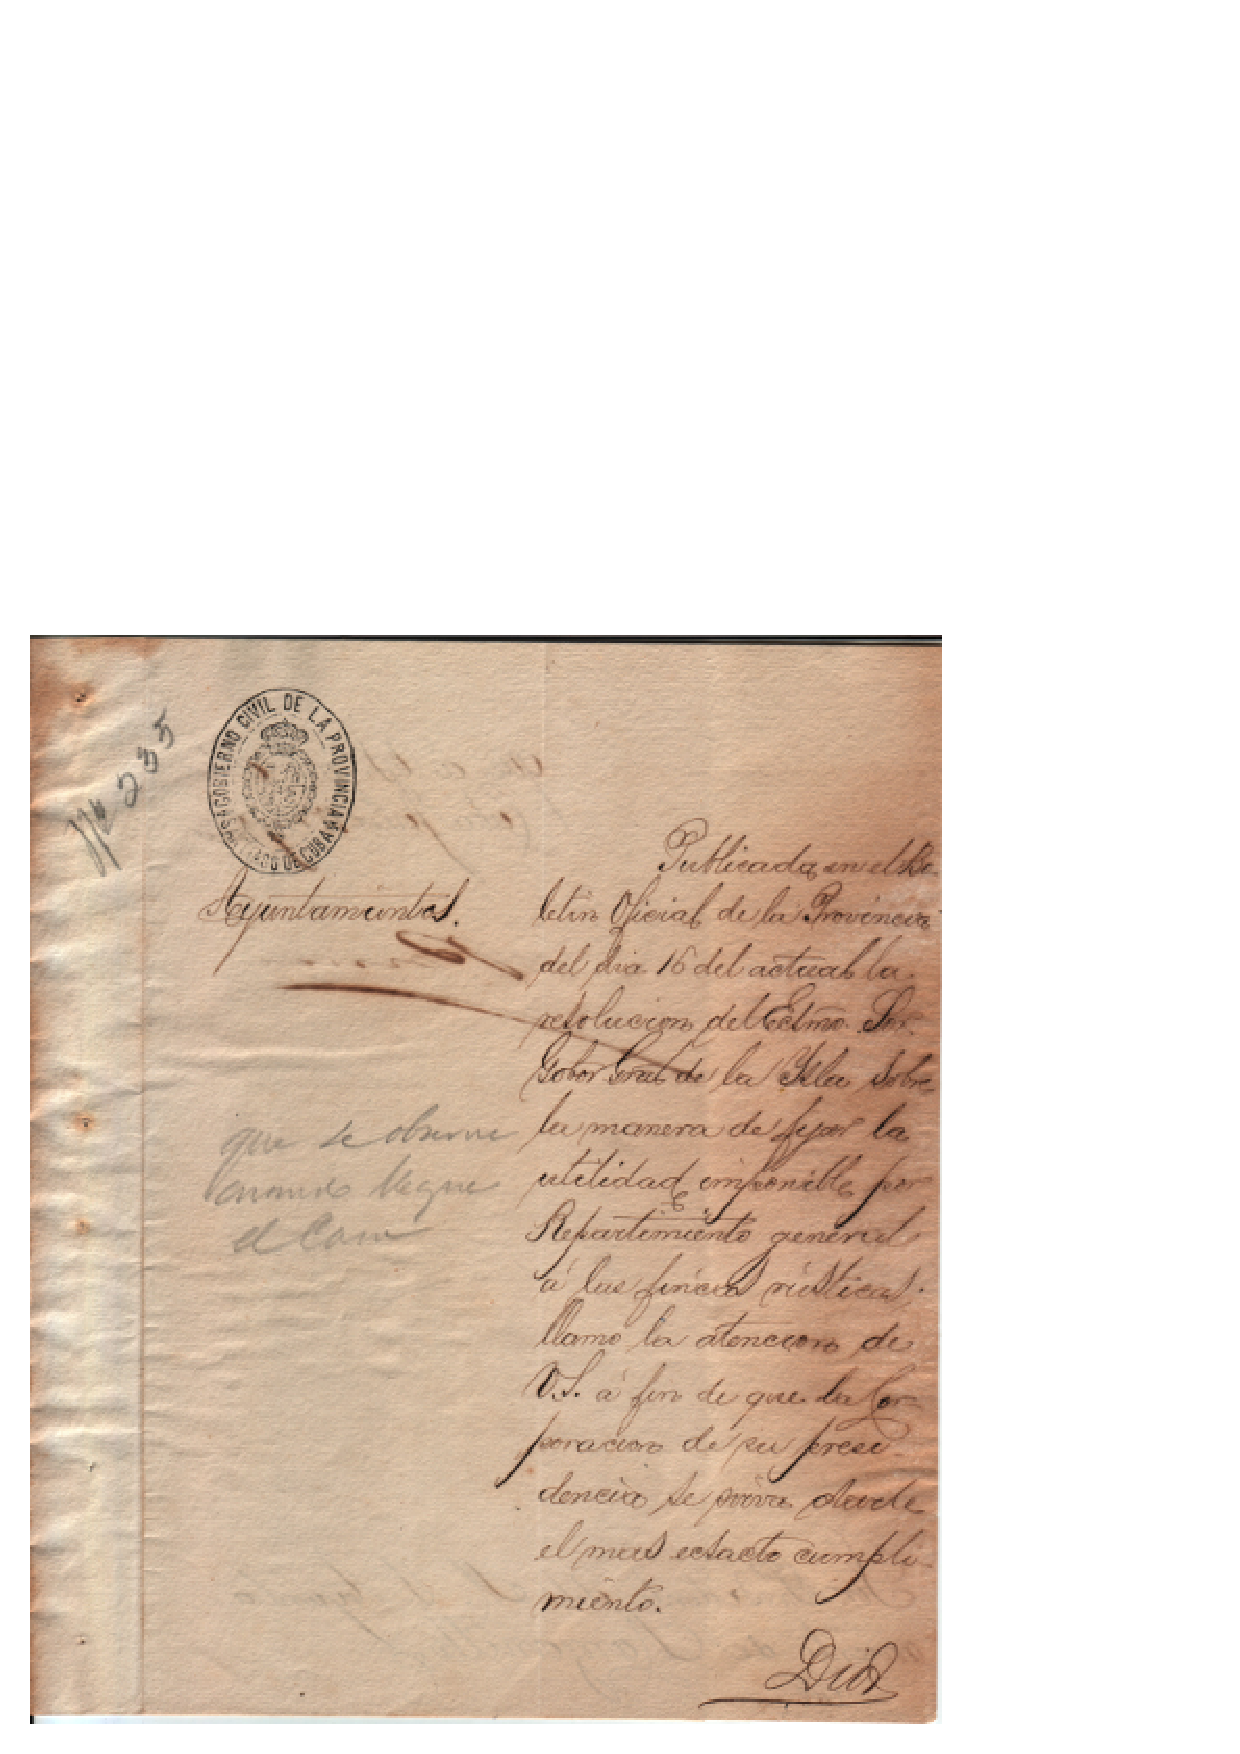
\includegraphics[width=0.25\textwidth]{1.jpg}
			&\includegraphics[width=0.25\textwidth]{watermarked_image.png}
			&\includegraphics[width=0.25\textwidth]{watermarked_image_with_noise.png}
			&\includegraphics[width=0.25\textwidth]{tampered_image.png}\\\hline
		\end{tabular}
	\end{center}
	\caption{Original image, watermarked image (PSNR 62.18), watermarked modified image and tamper area detection.}
	\label{img_of_AHM}
\end{figure}

\subsection{Robustness}
The bit error rate (BER) is defined as ratio between number of incorrectly decoded bits and total number of bits.

\begin{table}
\caption{Table captions should be placed above the
tables.}\label{tab1}
\begin{tabular}{|l|l|l|}
\hline
Heading level &  Example & Font size and style\\
\hline
Title (centered) &  {\Large\bfseries Lecture Notes} & 14 point, bold\\
1st-level heading &  {\large\bfseries 1 Introduction} & 12 point, bold\\
2nd-level heading & {\bfseries 2.1 Printing Area} & 10 point, bold\\
3rd-level heading & {\bfseries Run-in Heading in Bold.} Text follows & 10 point, bold\\
4th-level heading & {\itshape Lowest Level Heading.} Text follows & 10 point, italic\\
\hline
\end{tabular}
\end{table}


\noindent Displayed equations are centered and set on a separate
line.
\begin{equation}
x + y = z
\end{equation}
Please try to avoid rasterized images for line-art diagrams and
schemas. Whenever possible, use vector graphics instead (see
Fig.~\ref{fig1}).

\begin{figure}
\includegraphics[width=\textwidth]{fig1.eps}
\caption{A figure caption is always placed below the illustration.
Please note that short captions are centered, while long ones are
justified by the macro package automatically.} \label{fig1}
\end{figure}

\begin{theorem}
This is a sample theorem. The run-in heading is set in bold, while
the following text appears in italics. Definitions, lemmas,
propositions, and corollaries are styled the same way.
\end{theorem}
%
% the environments 'definition', 'lemma', 'proposition', 'corollary',
% 'remark', and 'example' are defined in the LLNCS documentclass as well.
%
\begin{proof}
Proofs, examples, and remarks have the initial word in italics,
while the following text appears in normal font.
\end{proof}
\section{Conclusions}
In this paper, a digital watermarking technique based on Krawtchouk moments was implemented, and it was optimized by a genetic algorithm for manuscript document images. The results show a BER less than $0.005 \%$, so the extracted QR codes were decoded in $100\%$ of the $60$ analyzed images. In addition, the values of PSNR in all cases exceeded $44dB$. Thus, there is no visual difference between the original and watermarked images.
%
% ---- Bibliography ----
%
% BibTeX users should specify bibliography style 'splncs04'.
% References will then be sorted and formatted in the correct style.
%
\bibliographystyle{splncs04}
\bibliography{mybibliography}
%
\end{document}
